\titre{Proposition} : Une proposition ou énoncé ou affirmation est ce qui est vrai ou faux. \\

\titre{Opérateurs} : $\daleth, \vee, \wedge, \rightarrow, \leftrightarrow$\\

\titre{Séparateurs} : $(,),\{,\},[,]$\\

\titre{Formules bien formées (fbf ou wff) }: C'est le plus petit ensemble tel que : 
\begin{itemize}
	\item Toute proposition est une formule (\titre{formule atomique})
	\item Si $A$ et $B$ sont des formules, alors : \\$\daleth A, (A\vee B), (A\wedge B), (A \rightarrow B), (A\leftrightarrow B)$ sont des formules.
\end{itemize}

\titre{Attention} Ne pas confondre langage et méta-langage. \\

\titre{Représentation arborescente} (exemple : $(p\wedge (q\vee r))$ )\\
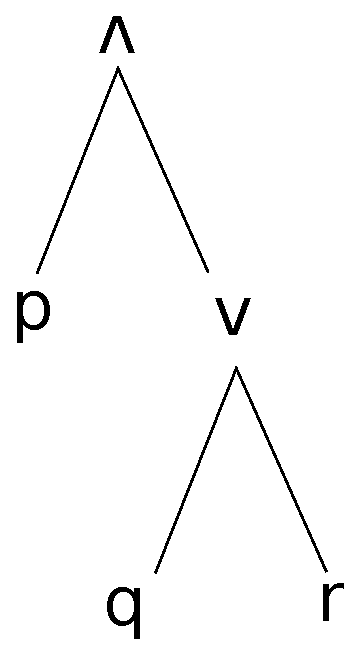
\includegraphics[width=0.15\linewidth]{fig2_arbo.pdf}
